%!TEX root = ./soutenance.tex


\section{Conception d'architectures programmables}



\subsection*{Conception d'architectures programmables}


\begin{frame}[c]{Spécialisation d'un processeur de base}
  \centering
  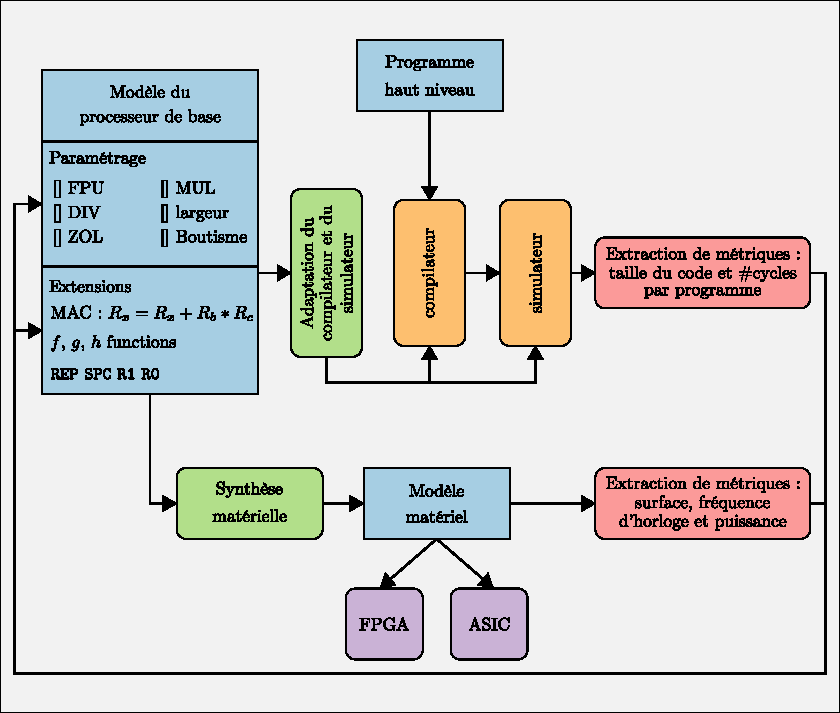
\includegraphics[width=0.7\textwidth]{./fig/methodos-1}
\end{frame}

\begin{frame}[c]{Spécialisation d'un processeur de base}
\renewcommand{\section}[2]{} % Trick to avoid references section

  \begin{columns}
    \begin{column}{.40\textwidth}
    \vspace{-1cm}
      \begin{itemize}
        \item Spécialisation d'un processeur de base
        \item Basé sur une architecture RISC
        \item Instructions spécialisées
        \item<2-> Réduction de la consommation énergétique
        \item<2-> Publication \color{bluecite}{\cite{leonardon_custom_2018}}
  
      \end{itemize}
    \end{column}
    \begin{column}[T]{.60\textwidth}
    \vspace{-0.5cm}

  \begin{minipage}[c][0cm][t]{\textwidth}

    \only<+>
    { 

      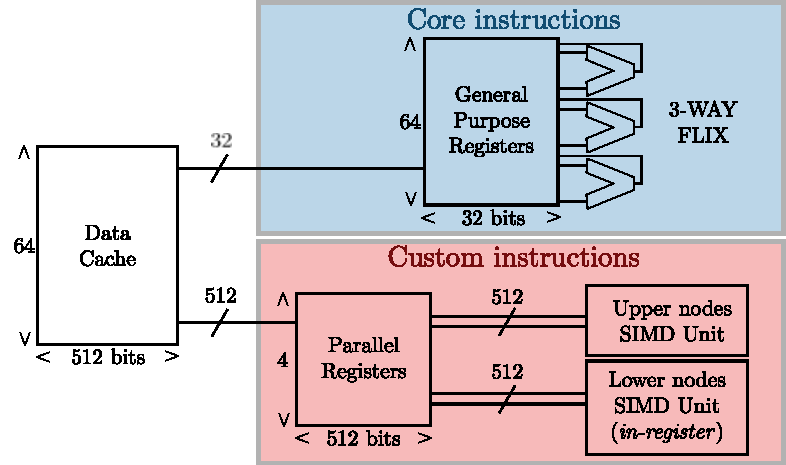
\includegraphics[width=\textwidth]{./fig/archi_tensilica}
    }
    \only<+->
    {
    \begin{table}[t]
      \centering
      {\small\resizebox{0.9\linewidth}{!}{
      \begin{tabular}{c|c|c|c|c}
        \toprule

        Cible & $N$ & \begin{tabular}{c}Latency\\{[$\mu$s]}\end{tabular} & \begin{tabular}{c}Throughput\\{[Mb/s]}\end{tabular} & \begin{tabular}{c}$E_b$\\{[nJ]}\end{tabular} \\

        \cmidrule(lr){1-1}
        \cmidrule(lr){2-2}
        \cmidrule(lr){3-5}
%                       
        \multirow{4}{*}{\bf A57-1.1GHz}  & $1024$   & $13$  & $38$  & \ORANGE{$\mathbf{21}$} \\

                                         & $512$    & $6.7$ & $38$  & \ORANGE{$\mathbf{21}$} \\

                                         & $256$    & $3.6$ & $35$  & \ORANGE{$\mathbf{22}$}\\

                                         & $128$    & $2.1$ & $30$  & \ORANGE{$\mathbf{27}$}\\

        \midrule

        \multirow{4}{*}{\bf i7-3.3GHz}   & $1024$   & $2.3$ & $222$ & \RED{$\mathbf{47}$} \\

                                         & $512$    & $1.4$ & $182$ & \RED{$\mathbf{57}$} \\

                                         & $256$    & $0.8$ & $155$ & \RED{$\mathbf{68}$}\\

                                         & $128$    & $0.5$ & $124$ & \RED{$\mathbf{85}$}\\

        \midrule

        \multirow{4}{*}{\bf ASIP-835MHz} & $1024$   & $7.2$ & $71$  & \GREEN{$\mathbf{1.6}$} \\

                                         & $512$    & $3.9$ & $66$  & \GREEN{$\mathbf{1.7}$} \\

                                         & $256$    & $1.9$ & $65$  & \GREEN{$\mathbf{1.7}$}\\

                                         & $128$    & $1.0$ & $62$  & \GREEN{$\mathbf{1.8}$}\\
        \bottomrule
      \end{tabular}
      }}
    \end{table}
    }
  \end{minipage} 
    \end{column}
  \end{columns}
\vfill
\centering
  \begin{minipage}[c][0cm][t]{\textwidth}
\only<2>
{
\renewcommand*{\bibfont}{\footnotesize}
    \printbibliography[keyword={leonardon}]

}
  \end{minipage} 
\end{frame}

\begin{frame}[c]{Définition complète d'une architecture de processeur}
  \centering
  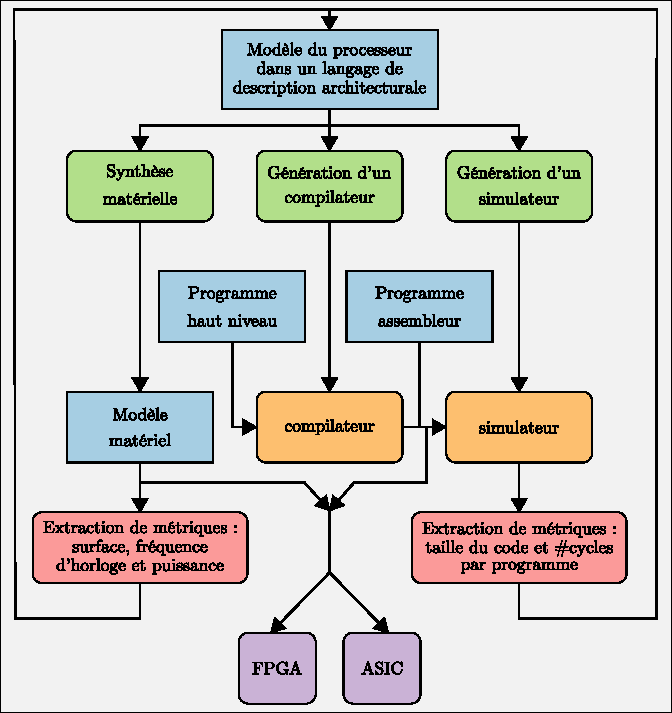
\includegraphics[width=0.5\textwidth]{./fig/methodos-2}
\end{frame}

\begin{frame}[c]{Transport Triggered Architectures}
  \begin{itemize}
    \vfill
    \item Modèle de processeur
    \vfill
    \item Similaire aux architectures VLIW
    \vfill
    \item Parallélisme de données
    \vfill
    \item Parallélisme d'instructions
    \vfill
  \end{itemize}
\end{frame}

\begin{frame}[c]{Structure d'un processeur TTA}
\centering
  \multiinclude[<+>][start=1,format=pdf,graphics={width=.8\textwidth}]{./fig/anim_tta_base}
\end{frame}

\begin{frame}[c]{Niveau de parallélisme}
  \centering
  \vfill
  Deux principales fonctions polaires : $f$ and $g$
  \vfill
  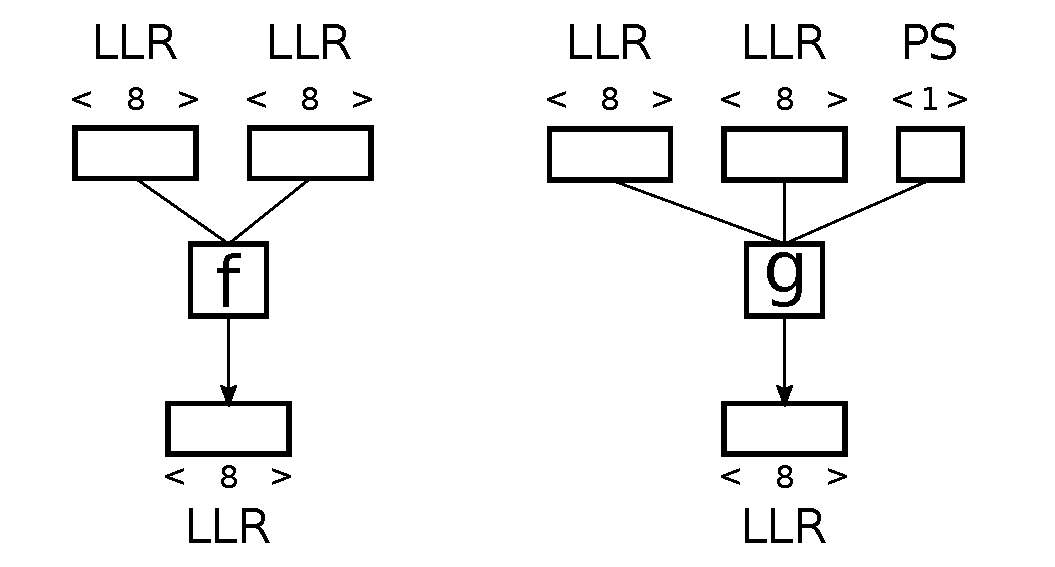
\includegraphics[width=0.7\textwidth]{fig/f_g_dimensions_scalar}
  \vfill
\end{frame}

\begin{frame}[c,noframenumbering]{Niveau de parallélisme}
  \centering
  \vfill
  Deux principales fonctions polaires : $f$ and $g$
  \vfill
  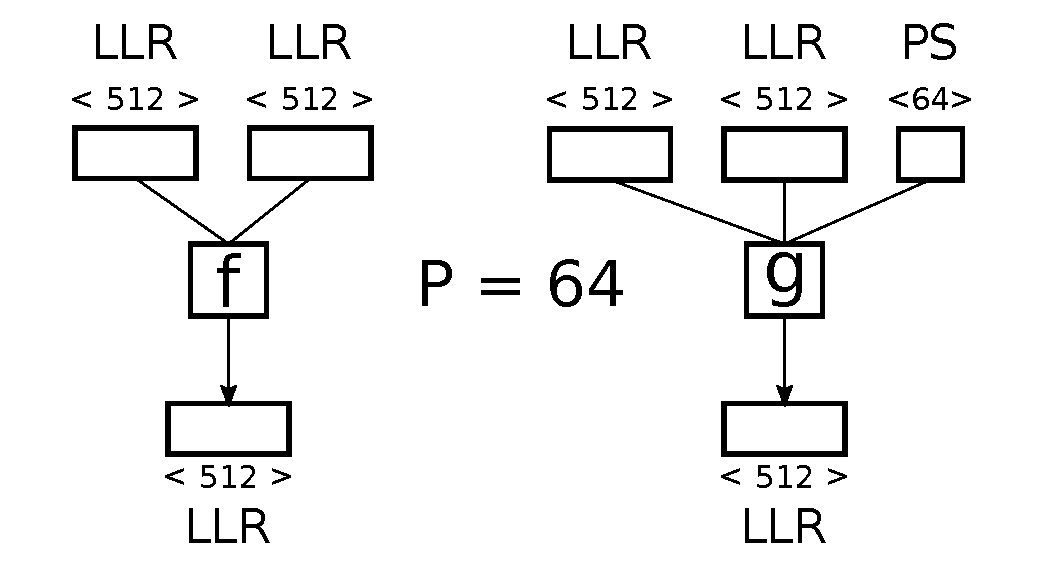
\includegraphics[width=0.7\textwidth]{fig/f_g_dimensions_vector}
  \vfill
\end{frame}

\begin{frame}[c]{Conception du processeur}
  \begin{columns}[T] % align columns
    \begin{column}{.48\textwidth}
      \vspace{-0.5cm}
      \multiinclude[<+>][start=1,format=pdf,graphics={width=1.4\textwidth}]{./fig/archi_sc_construction}
    \end{column}
    \begin{column}{.07\textwidth}
    \end{column}
    \begin{column}{.41\textwidth}
      \begin{itemize}
        \item<1-> Mémoires vectorielles
        \vspace{0.2cm}
        \item<2-> 2 bus de 512 bits
        \vspace{0.2cm}
        \item<2-> 1 bus de 64 bits
        \vspace{0.2cm}
        \item<3-> Unité de chargement et sauvegarde vectorielles
        \vspace{0.2cm}
        \item<4-> Unité de calcul polaire
      \end{itemize}
    \end{column}
  \end{columns} % align columns
\end{frame}

\begin{frame}[c]{Compilation}
  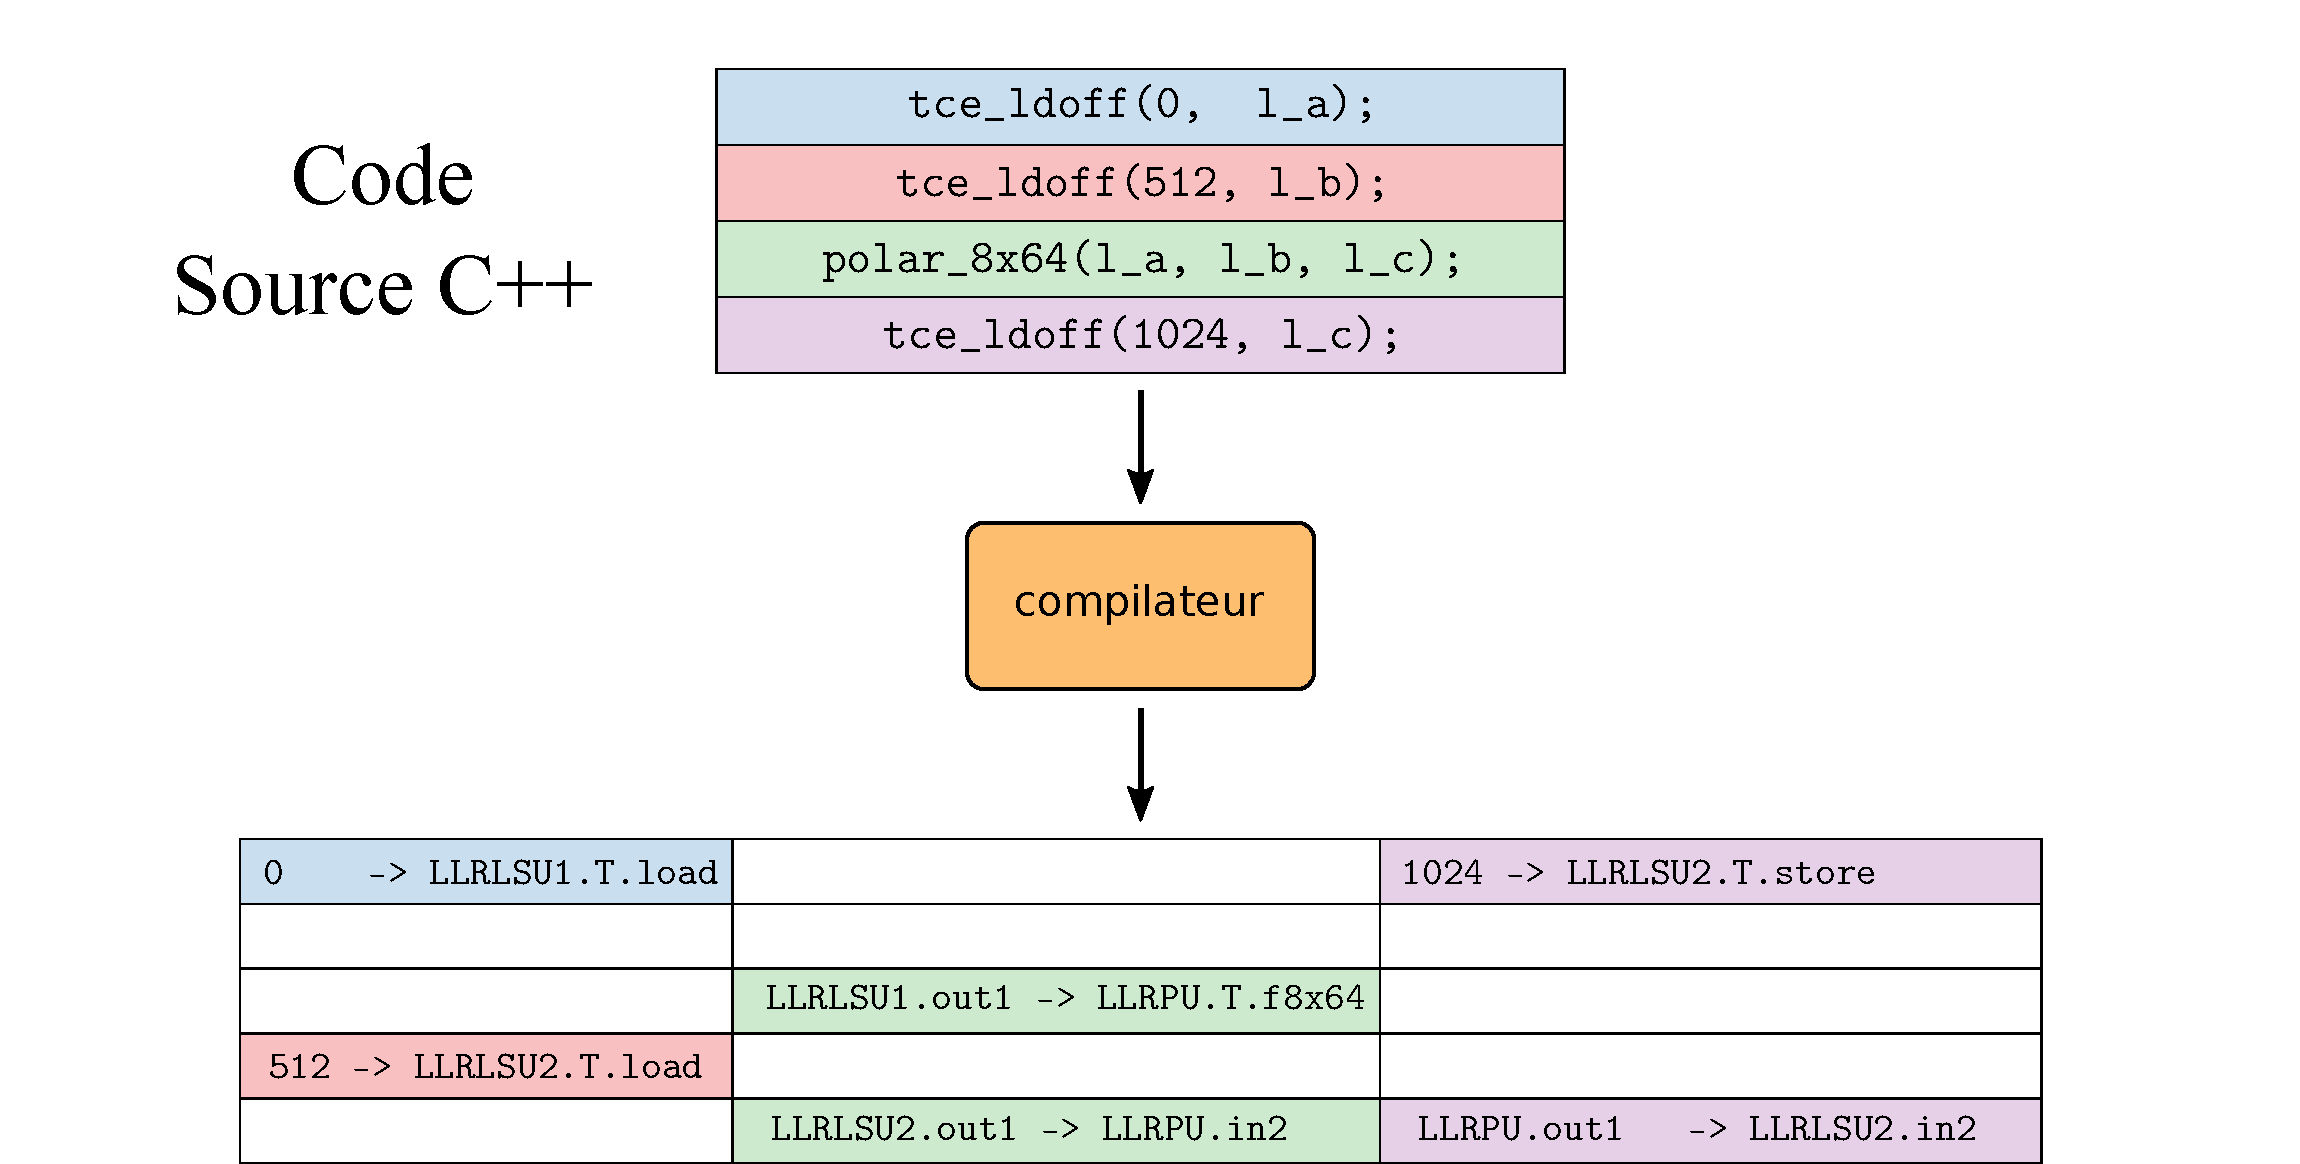
\includegraphics[width=\textwidth]{fig/compilation}
\end{frame}

\begin{frame}[c]{Comparaison avec des décodeurs logiciels}
  \begin{columns}[T] % align columns
  \begin{column}{.48\textwidth}
    \begin{itemize}
      \vfill
      \item<+-> Processeurs Intel x86 (i7-4712HQ) et ARM (Cortex A57)
      \vfill
      \item<+-> ASIP de type Tensilica
      \vfill
      \item<+-> Architecture TTA
      \vfill
      \item<+-> Débit maximum atteint par le processeur TTA
      \vfill
      \item<+-> Consommation énergétique réduite d'un à deux ordres de grandeur
      \vfill
    \end{itemize}
  \end{column}

  \begin{column}{.48\textwidth}
  \only<3>{
    \begin{table}
      \centering
      {
      \small\resizebox{\linewidth}{!}{
      \begin{tabular}{c|c|c|c|c}
        \toprule

        Architecture & $N$ & \begin{tabular}{c}Latence\\{[$\mu$s]}\end{tabular} & \begin{tabular}{c}Débit\\{[Mb/s]}\end{tabular} & \begin{tabular}{c}$E_b$\\{[nJ/bit]}\end{tabular} \\

        \cmidrule(lr){1-1}
        \cmidrule(lr){2-2}
        \cmidrule(lr){3-5}

        \multirow{2}{*}{\bf i7-3.3GHz}              & $1024$   & $2.0$  & $257$ & $41$   \\
                                                    & $512$    & $1.2$  & $210$ & $49$   \\
        \multirow{2}{*}{\bf (GPP)}                  & $256$    & $0.7$  & $179$ & $59$   \\
                                                    & $128$    & $0.4$  & $143$ & $73$   \\
        \midrule    
        \multirow{2}{*}{\bf A57-1.1GHz}             & $1024$   & $10.7$ & $48$  & $17$   \\
                                                    & $512$    & $5.3$  & $48$  & $17$   \\
        \multirow{2}{*}{\bf (GPP)}                  & $256$    & $2.8$  & $46$  & $17$   \\
                                                    & $128$    & $1.6$  & $41$  & $20$   \\
        \midrule
        \multirow{2}{*}{\bf LX7-835MHz}             & $1024$   & $7.2$  & $71$  & $1.6$  \\
                                                    & $512$    & $3.9$  & $66$  & $1.7$  \\
        \multirow{2}{*}{\bf (ASIP)}                 & $256$    & $1.9$  & $65$  & $1.7$  \\
                                                    & $128$    & $1.0$  & $62$  & $1.8$  \\
        \midrule
        \multirow{2}{*}{\bf \BLUE{TTPD-800MHz}}     & $1024$   & $1.4$  & $352$ & $0.14$ \\ % 1512 cycles
                                                    & $512$    & $0.8$  & $313$ & $0.15$ \\ % 803 cycles
        \multirow{2}{*}{\bf \BLUE{(ASIP)}}          & $256$    & $0.4$  & $304$ & $0.16$ \\ % 413 cycles
                                                    & $128$    & $0.2$  & $284$ & $0.17$ \\ % 224 cycles
        \bottomrule
      \end{tabular}
      }}
    \end{table}
  }
    
    \only<1>{
    \begin{table}
      \centering
      {
      \small\resizebox{\linewidth}{!}{
      \begin{tabular}{c|c|c|c|c}
        \toprule

        Architecture & $N$ & \begin{tabular}{c}Latence\\{[$\mu$s]}\end{tabular} & \begin{tabular}{c}Débit\\{[Mb/s]}\end{tabular} & \begin{tabular}{c}$E_b$\\{[nJ/bit]}\end{tabular} \\

        \cmidrule(lr){1-1}
        \cmidrule(lr){2-2}
        \cmidrule(lr){3-5}


        \multirow{2}{*}{\bf \BLUE{i7-3.3GHz}}       & $1024$   & $2.0$  & $257$ & $41$   \\
                                                    & $512$    & $1.2$  & $210$ & $49$   \\
        \multirow{2}{*}{\bf \BLUE{(GPP)}}           & $256$    & $0.7$  & $179$ & $59$   \\
                                                    & $128$    & $0.4$  & $143$ & $73$   \\
        \midrule    
        \multirow{2}{*}{\bf \BLUE{A57-1.1GHz}}      & $1024$   & $10.7$ & $48$  & $17$   \\
                                                    & $512$    & $5.3$  & $48$  & $17$   \\
        \multirow{2}{*}{\bf \BLUE{(GPP)}}           & $256$    & $2.8$  & $46$  & $17$   \\
                                                    & $128$    & $1.6$  & $41$  & $20$   \\
        \midrule
        \multirow{2}{*}{\bf LX7-835MHz}             & $1024$   & $7.2$  & $71$  & $1.6$  \\
                                                    & $512$    & $3.9$  & $66$  & $1.7$  \\
        \multirow{2}{*}{\bf (ASIP)}                 & $256$    & $1.9$  & $65$  & $1.7$  \\
                                                    & $128$    & $1.0$  & $62$  & $1.8$  \\
        \midrule
        \multirow{2}{*}{\bf TTPD-800MHz}            & $1024$   & $1.4$  & $352$ & $0.14$ \\ % 1512 cycles
                                                    & $512$    & $0.8$  & $313$ & $0.15$ \\ % 803 cycles
        \multirow{2}{*}{\bf (ASIP)}                 & $256$    & $0.4$  & $304$ & $0.16$ \\ % 413 cycles
                                                    & $128$    & $0.2$  & $284$ & $0.17$ \\ % 224 cycles
        \bottomrule
      \end{tabular}
      }}
    \end{table}
    }

  \only<2>{
    \begin{table}
      \centering
      {
      \small\resizebox{\linewidth}{!}{
      \begin{tabular}{c|c|c|c|c}
        \toprule

        Architecture & $N$ & \begin{tabular}{c}Latence\\{[$\mu$s]}\end{tabular} & \begin{tabular}{c}Débit\\{[Mb/s]}\end{tabular} & \begin{tabular}{c}$E_b$\\{[nJ/bit]}\end{tabular} \\

        \cmidrule(lr){1-1}
        \cmidrule(lr){2-2}
        \cmidrule(lr){3-5}


        \multirow{2}{*}{\bf i7-3.3GHz}              & $1024$   & $2.0$  & $257$ & $41$   \\
                                                    & $512$    & $1.2$  & $210$ & $49$   \\
        \multirow{2}{*}{\bf (GPP)}                  & $256$    & $0.7$  & $179$ & $59$   \\
                                                    & $128$    & $0.4$  & $143$ & $73$   \\
        \midrule    
        \multirow{2}{*}{\bf A57-1.1GHz}             & $1024$   & $10.7$ & $48$  & $17$   \\
                                                    & $512$    & $5.3$  & $48$  & $17$   \\
        \multirow{2}{*}{\bf (GPP)}                  & $256$    & $2.8$  & $46$  & $17$   \\
                                                    & $128$    & $1.6$  & $41$  & $20$   \\
        \midrule
        \multirow{2}{*}{\bf \BLUE{LX7-835MHz}}      & $1024$   & $7.2$  & $71$  & $1.6$  \\
                                                    & $512$    & $3.9$  & $66$  & $1.7$  \\
        \multirow{2}{*}{\bf \BLUE{(ASIP)}}          & $256$    & $1.9$  & $65$  & $1.7$  \\
                                                    & $128$    & $1.0$  & $62$  & $1.8$  \\
        \midrule
        \multirow{2}{*}{\bf TTPD-800MHz}            & $1024$   & $1.4$  & $352$ & $0.14$ \\ % 1512 cycles
                                                    & $512$    & $0.8$  & $313$ & $0.15$ \\ % 803 cycles
        \multirow{2}{*}{\bf (ASIP)}                 & $256$    & $0.4$  & $304$ & $0.16$ \\ % 413 cycles
                                                    & $128$    & $0.2$  & $284$ & $0.17$ \\ % 224 cycles

        \bottomrule
      \end{tabular}
      }}
    \end{table}
    }
    \only<4>{
    \begin{table}
      \centering
      {
      \small\resizebox{\linewidth}{!}{
      \begin{tabular}{c|c|c|c|c}
        \toprule

        Architecture & $N$ & \begin{tabular}{c}Latence\\{[$\mu$s]}\end{tabular} & \begin{tabular}{c}Débit\\{[Mb/s]}\end{tabular} & \begin{tabular}{c}$E_b$\\{[nJ/bit]}\end{tabular} \\

        \cmidrule(lr){1-1}
        \cmidrule(lr){2-2}
        \cmidrule(lr){3-5}


        \multirow{2}{*}{\bf i7-3.3GHz}              & $1024$   & $2.0$  & \GREEN{$\mathbf{257}$} & $41$   \\
                                                    & $512$    & $1.2$  & \GREEN{$\mathbf{210}$} & $49$   \\
        \multirow{2}{*}{\bf (GPP)}                  & $256$    & $0.7$  & \GREEN{$\mathbf{179}$} & $59$   \\
                                                    & $128$    & $0.4$  & \GREEN{$\mathbf{143}$} & $73$   \\
        \midrule    
        \multirow{2}{*}{\bf A57-1.1GHz}             & $1024$   & $10.7$ & \ORANGE{$\mathbf{48}$} & $17$   \\
                                                    & $512$    & $5.3$  & \ORANGE{$\mathbf{48}$} & $17$   \\
        \multirow{2}{*}{\bf (GPP)}                  & $256$    & $2.8$  & \ORANGE{$\mathbf{46}$} & $17$   \\
                                                    & $128$    & $1.6$  & \ORANGE{$\mathbf{41}$} & $20$   \\
        \midrule
        \multirow{2}{*}{\bf LX7-835MHz}             & $1024$   & $7.2$  & \ORANGE{$\mathbf{71}$} & $1.6$  \\
                                                    & $512$    & $3.9$  & \ORANGE{$\mathbf{66}$} & $1.7$  \\
        \multirow{2}{*}{\bf (ASIP)}                 & $256$    & $1.9$  & \ORANGE{$\mathbf{65}$} & $1.7$  \\
                                                    & $128$    & $1.0$  & \ORANGE{$\mathbf{62}$} & $1.8$  \\
        \midrule
        \multirow{2}{*}{\bf TTPD-800MHz}            & $1024$   & $1.4$  & \GREEN{$\mathbf{352}$} & $0.14$ \\ % 1512 cycles
                                                    & $512$    & $0.8$  & \GREEN{$\mathbf{313}$} & $0.15$ \\ % 803 cycles
        \multirow{2}{*}{\bf (ASIP)}                 & $256$    & $0.4$  & \GREEN{$\mathbf{304}$} & $0.16$ \\ % 413 cycles
                                                    & $128$    & $0.2$  & \GREEN{$\mathbf{284}$} & $0.17$ \\ % 224 cycles

        \bottomrule
      \end{tabular}
      }}
    \end{table}
    }
    \only<5>{
    \begin{table}
      \centering
      {
      \small\resizebox{\linewidth}{!}{
      \begin{tabular}{c|c|c|c|c}
        \toprule

        Architecture & $N$ & \begin{tabular}{c}Latence\\{[$\mu$s]}\end{tabular} & \begin{tabular}{c}Débit\\{[Mb/s]}\end{tabular} & \begin{tabular}{c}$E_b$\\{[nJ/bit]}\end{tabular} \\

        \cmidrule(lr){1-1}
        \cmidrule(lr){2-2}
        \cmidrule(lr){3-5}


        \multirow{2}{*}{\bf i7-3.3GHz}              & $1024$   & $2.0$  & $257$ & \RED{$\mathbf{41}$}   \\
                                                    & $512$    & $1.2$  & $210$ & \RED{$\mathbf{49}$}   \\
        \multirow{2}{*}{\bf (GPP)}                  & $256$    & $0.7$  & $179$ & \RED{$\mathbf{59}$}   \\
                                                    & $128$    & $0.4$  & $143$ & \RED{$\mathbf{73}$}   \\
        \midrule    
        \multirow{2}{*}{\bf A57-1.1GHz}             & $1024$   & $10.7$ & $48$  & \RED{$\mathbf{17}$}   \\
                                                    & $512$    & $5.3$  & $48$  & \RED{$\mathbf{17}$}   \\
        \multirow{2}{*}{\bf (GPP)}                  & $256$    & $2.8$  & $46$  & \RED{$\mathbf{17}$}   \\
                                                    & $128$    & $1.6$  & $41$  & \RED{$\mathbf{20}$}   \\
        \midrule
        \multirow{2}{*}{\bf LX7-835MHz}             & $1024$   & $7.2$  & $71$  & \ORANGE{$\mathbf{1.6}$}  \\
                                                    & $512$    & $3.9$  & $66$  & \ORANGE{$\mathbf{1.7}$}  \\
        \multirow{2}{*}{\bf (ASIP)}                 & $256$    & $1.9$  & $65$  & \ORANGE{$\mathbf{1.7}$}  \\
                                                    & $128$    & $1.0$  & $62$  & \ORANGE{$\mathbf{1.8}$}  \\
        \midrule
        \multirow{2}{*}{\bf TTPD-800MHz}            & $1024$   & $1.4$  & $352$ & \GREEN{$\mathbf{0.14}$} \\ % 1512 cycles
                                                    & $512$    & $0.8$  & $313$ & \GREEN{$\mathbf{0.15}$} \\ % 803 cycles
        \multirow{2}{*}{\bf (ASIP)}                 & $256$    & $0.4$  & $304$ & \GREEN{$\mathbf{0.16}$} \\ % 413 cycles
                                                    & $128$    & $0.2$  & $284$ & \GREEN{$\mathbf{0.17}$} \\ % 224 cycles

        \bottomrule
      \end{tabular}
      }}
    \end{table}
    }
  \end{column}
  \end{columns}
\end{frame}

\begin{frame}[c]{Comparaison avec des architectures matérielles dédiées}
    \begin{itemize}
      \item<+-> Transport Triggered Polar Decoder
      \item<+-> Architecture matérielle dédiée 
      \item<2-> Architecture matérielle dédiée avec bits gelés adaptés
      \item<+-> Implémentations FPGA
    \end{itemize}

    \only<1>{
      \begin{table}
      \centering
      {
        \small\resizebox{1\linewidth}{!}{
        \begin{tabular}{C{3cm}|C{3cm}|C{2cm}|C{2cm}}
                                  & \BLUE{TTPD}  & \cite{giard_638_2015} & \cite{sarkis2014fast} \\
          \cmidrule(lr){1-1}
          \cmidrule(lr){2-2}
          \cmidrule(lr){3-3}
          \cmidrule(lr){4-4}

          \textbf{Cible}         &  Stratix IV       & Stratix IV            & Stratix IV     \\
          \textbf{RAM} (Kb)       &  141           & 43                    & 36               \\
          \textbf{LUTS}           &  19664         & 23020                 & 24821            \\
          \textbf{\'Elagage}        &  R0 \& R1      & Full                  & Full           \\
          \textbf{Cycles d'horloge}   &  1161          & 222                   & 165          \\

        \end{tabular}
      }}
      \end{table}
    }

    \only<2>{
      \begin{table}
      \centering
      {
        \small\resizebox{1\linewidth}{!}{
        \begin{tabular}{C{3cm}|C{3cm}|C{2cm}|C{2cm}}
                                  & TTPD  & \BLUE{\cite{giard_638_2015}} & \BLUE{\cite{sarkis2014fast}} \\
          \cmidrule(lr){1-1}
          \cmidrule(lr){2-2}
          \cmidrule(lr){3-3}
          \cmidrule(lr){4-4}

          \textbf{Cible}         &  Stratix IV       & Stratix IV            & Stratix IV                 \\
          \textbf{RAM} (Kb)       &  141           & 43                    & 36                         \\
          \textbf{LUTS}           &  19664         & 23020                 & 24821                      \\
          \textbf{\'Elagage}        &  R0 \& R1      & Full                  & Full                       \\
          \textbf{Cycles d'horloge}   &  1161          & 222                   & 165                        \\

        \end{tabular}
      }}
      \end{table}
    }

    \only<3>{
      \begin{table}
      \centering
      {
        \small\resizebox{1\linewidth}{!}{
        \begin{tabular}{C{3cm}|C{3cm}|C{2cm}|C{2cm}}
                                  & TTPD  & \cite{giard_638_2015} & \cite{sarkis2014fast} \\
          \cmidrule(lr){1-1}
          \cmidrule(lr){2-2}
          \cmidrule(lr){3-3}
          \cmidrule(lr){4-4}

          \textbf{Cible}         &  \BLUE{Stratix IV}       & \textbf{Stratix IV}            & \textbf{Stratix IV }            \\
          \textbf{RAM} (Kb)       &  141           & 43                    & 36                           \\
          \textbf{LUTS}           &  19664         & 23020                 & 24821                        \\
          \textbf{\'Elagage}        &  R0 \& R1      & Full                  & Full                         \\
          \textbf{Cycles d'horloge}   &  1161          & 222                   & 165                          \\

        \end{tabular}
      }}
      \end{table}
    }
\end{frame}

\begin{frame}[c,noframenumbering]{Comparaison avec des architectures matérielles dédiées}
    \begin{itemize}
      \item<+-> Empreinte mémoire plus importante
      \item<+-> Nombre inférieur de LUTs
      \item<+-> \'Elagage différent
      \item<+-> 5 à 7 fois plus de cycles d'horloge
    \end{itemize}
    \only<1>{
      \begin{table}
      \centering
      {
        \small\resizebox{1\linewidth}{!}{
        \begin{tabular}{C{3cm}|C{3cm}|C{2cm}|C{2cm}}
                                  & TTPD  & \cite{giard_638_2015} & \cite{sarkis2014fast} \\
          \cmidrule(lr){1-1}
          \cmidrule(lr){2-2}
          \cmidrule(lr){3-3}
          \cmidrule(lr){4-4}

          \textbf{Cible}         &  Stratix IV       & Stratix IV            & Stratix IV                 \\
          \textbf{RAM} (Kb)       &  \textbf{141}  & \textbf{43}           & \textbf{36}                \\
          \textbf{LUTS}           &  19664         & 23020                 & 24821                      \\
          \textbf{\'Elagage}        &  R0 \& R1      & Full                  & Full                        \\
          \textbf{Cycles d'horloge}   &  1161          & 222                   & 165                        \\


        \end{tabular}
      }}
      \end{table}
    }
    \only<2>{
      \begin{table}
      \centering
      {
        \small\resizebox{1\linewidth}{!}{
        \begin{tabular}{C{3cm}|C{3cm}|C{2cm}|C{2cm}}
                                  & TTPD  & \cite{giard_638_2015} & \cite{sarkis2014fast} \\
          \cmidrule(lr){1-1}
          \cmidrule(lr){2-2}
          \cmidrule(lr){3-3}
          \cmidrule(lr){4-4}

          \textbf{Cible}         &  Stratix IV        & Stratix IV             & Stratix IV                \\
          \textbf{RAM} (Kb)       &  141            & 43                     & 36                        \\
          \textbf{LUTS}           &  \textbf{19664} & \textbf{23020}         & \textbf{24821}            \\
          \textbf{\'Elagage}        &  R0 \& R1       & Full                   & Full                      \\
          \textbf{Cycles d'horloge}   &  1161           & 222                    & 165                       \\


        \end{tabular}
      }}
      \end{table}
    }
    \only<3>{
      \begin{table}
      \centering
      {
        \small\resizebox{1\linewidth}{!}{
        \begin{tabular}{C{3cm}|C{3cm}|C{2cm}|C{2cm}}
                                  & TTPD  & \cite{giard_638_2015} & \cite{sarkis2014fast} \\
          \cmidrule(lr){1-1}
          \cmidrule(lr){2-2}
          \cmidrule(lr){3-3}
          \cmidrule(lr){4-4}

          \textbf{Cible}         &  Stratix IV       & Stratix IV            & Stratix IV             \\
          \textbf{RAM} (Kb)       &  141           & 43                    & 36                     \\
          \textbf{LUTS}           &  19664         & 23020                 & 24821                  \\
          \textbf{\'Elagage}        &  \textbf{R0 \& R1}      & \textbf{Full}                             & \textbf{Full}                 \\
          \textbf{Cycles d'horloge}   &  1161          & 222                   & 165                    \\

        \end{tabular}
      }}
      \end{table}
    }

    \only<4>{
      \begin{table}
      \centering
      {
        \small\resizebox{1\linewidth}{!}{
        \begin{tabular}{C{3cm}|C{3cm}|C{2cm}|C{2cm}}
                                  & TTPD  & \cite{giard_638_2015} & \cite{sarkis2014fast} \\
          \cmidrule(lr){1-1}
          \cmidrule(lr){2-2}
          \cmidrule(lr){3-3}
          \cmidrule(lr){4-4}

          \textbf{Cible}         &  Stratix IV       & Stratix IV            & Stratix IV      \\
          \textbf{RAM} (Kb)       &  141           & 43                    & 36                \\
          \textbf{LUTS}           &  19664         & 23020                 & 24821             \\
          \textbf{\'Elagage}        &  R0 \& R1      & Full                  & Full            \\
          \textbf{Cycles d'horloge}   &  \textbf{1161} & \textbf{222}          & \textbf{165}  \\

        \end{tabular}
      }}
      \end{table}
    }
\end{frame}


\section{Conclusions et perspectives}
\subsection*{}

\begin{frame}[c]{Conclusions}

  \begin{enumerate}
\renewcommand{\section}[2]{} % Trick to avoid references section

    \renewcommand*{\bibfont}{\scriptsize}
    \nocite{leonardon_fast_2017,ghaffari_improving_2017,leonardon_tta_2018,Ghaffari2018,cassagne_fast_2017,cassagne_gdr_2017}
    \vfill
    \item<+-> Implémentation logicielle de l'algorithme  SCL
    \scriptsize{\printbibliography[keyword={fast-scl}]}
    \vfill
    \item<+-> Spécialisation d'un processeur Tensilica
    \scriptsize{\printbibliography[keyword={leonardon}]}
    \vfill
    \item<+-> Conception d'un processeur de type TTA
    \scriptsize{\printbibliography[keyword={tta}]}
    \vfill
  \end{enumerate}

\end{frame}

\begin{frame}[c]{Conclusions}

  \begin{enumerate}
\renewcommand{\section}[2]{} % Trick to avoid references section

    \renewcommand*{\bibfont}{\scriptsize}
    \nocite{leonardon_fast_2017,ghaffari_improving_2017,leonardon_tta_2018,Ghaffari2018,cassagne_fast_2017,cassagne_gdr_2017}
    \vfill
    \item<+-> Implémentation du décodeur SCMA
    \printbibliography[keyword={ghaffari}]
    \vfill
    \item<+-> Contribution au projet AFF3CT
    \printbibliography[keyword={aff3ct}]
    \vfill
  \end{enumerate}

\end{frame}

\begin{frame}[c]{Perspectives}

  \begin{itemize}
    \renewcommand*{\bibfont}{\scriptsize}
    \vfill
    \item<+-> Extension des travaux sur les décodeurs logiciels
    \begin{itemize}
      \item Implémentation logicielle de variantes algorithmiques
      \item Support de nouvelles constructions de codes polaires
    \end{itemize}
    \vfill
    \item<+-> Intégration des codes polaires dans des chaînes de communications plus complexes
    \begin{itemize}
      \item Travaux sur le SCMA
      \item Chaîne de réception 5G
    \end{itemize}
    \item<+-> Extension des travaux sur le TTA
    \begin{itemize}
      \item Architecture pour le décodage à liste
      \item Architectures multicœurs
    \end{itemize}
    \vfill
    \vfill
  \end{itemize}

\end{frame}

\begin{frame}[c]{Merci}
\vfill
\centering
Merci pour votre attention !
\vfill
\end{frame}

\begin{frame}[allowframebreaks]{Références}
\renewcommand*{\bibfont}{\scriptsize}

\printbibliography
\end{frame}
